\section{结果讨论与工程验证}
\label{sec:discussion}
\subsection{匿名化与表情保持}
项目把面部区域控制与表情信息保留落实为两个相互配合的环节：局部掩膜控制修改边界，几何与关键点条件控制动作结构。匿名化不需要改变整幅图像，背景保持可以通过掩膜外像素直接核对；表情保持则通过匿名输入上的真实标签准确率评价。两者分别检查，使视觉效果与识别结果都有明确依据。

\subsection{统一模块的两种配置}
高速和质量配置共用匿名输入边界、标签顺序与结果接口。前者压低计算开销，适合持续观察；后者通过更完整的表征、翻转增强和概率校准提高离线识别质量。质量配置在 RAF-DB 上取得 78.39\% 的匿名图准确率，配合车载集合结果，为按使用场景选择运行开销提供依据。

\begin{figure}[htbp]
\centering
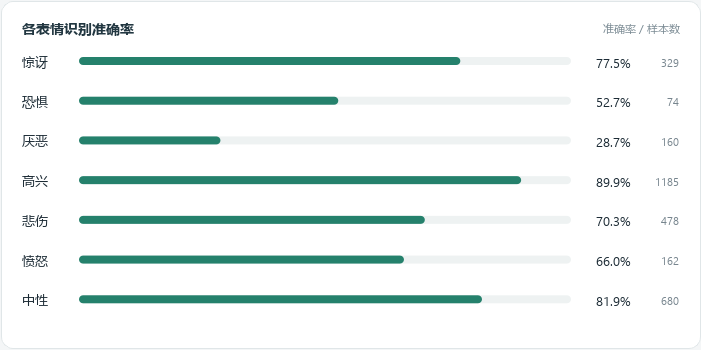
\includegraphics[width=.82\linewidth]{ui_performance_detail.png}
\caption{模型表现页中的类别统计区域}
\label{fig:uiperf}
\end{figure}

\subsection{输入边界与工程检查}
工程检查沿着数据流逐段开展：先核对灰度转换与人脸对齐，再核对匿名合成和分类器实参，最后核对页面显示、视频输出与记录。缓存中的源文件标识、匿名参数及输入来源用来追踪样本；模型契约中的文件校验值用来核对运行资源。检测或匿名化失败时不向分类器传入原脸，使输入边界在异常处理中仍然成立。

\subsection{近红外条件与实时策略}
视频采用检测结果复用、轨迹状态更新和因果概率平滑，减少重复计算与孤立跳变。置信度从匿名帧的模型概率得到，不按连续显示次数人为加分；轨迹变化后重建时序状态，使结果跟随当前画面。质量优先的选择保留在同一桌面入口中，用户可根据连续观察或离线分析的需求调整计算开销。
